El objetivo de la plan de gestión de riesgos es identificar, analizar y planificar la respuesta a los distintos riesgos a los que está expuesto el proyecto, de esta manera se busca minimizar la probabilidad de ocurrencia de los riesgos y reducir el impacto de los mismos en el proyecto.
\subsection*{Metodología aplicada}
Este plan se ha realizado siguiendo principalmente la metodología Boehm \cite{boehm1991} que divide la gestión de riesgos en dos fases: valoración de riesgos y control de riesgos. Cabe destacar que esta metodología ha sido adaptada a las necesidades del proyecto, añadiendo el paso previo de planificación según la metodología PMBOK \cite{pmbok2013}. De esta manera, finalmente tenemos tres fases:

\begin{itemize}
    \item \textbf{Planificar la gestión de riesgos:} Se definen los objetivos, alcance, metodología y responsabilidades.
    \item \textbf{Valoración de riesgos:} En esta fase se identifican los riesgos, se analizan y se priorizan.
    \item \textbf{Control de riesgos:} En esta fase se planifican las respuestas a los riesgos identificados en la fase anterior, la resolución de riesgos y la monitorización de estos.
\end{itemize}
\subsection*{Planificación de la gestión de riesgos}
\subsubsection*{Categorías de riesgos}
Basánsose en la estructura de desglose de riesgo representadas en el PMBOK, se han identificado las siguientes categorías de riesgos para el proyecto:

\begin{figure}[H]
    \hypertarget{fig:A1_PGR_RBS}{}
    \centering
    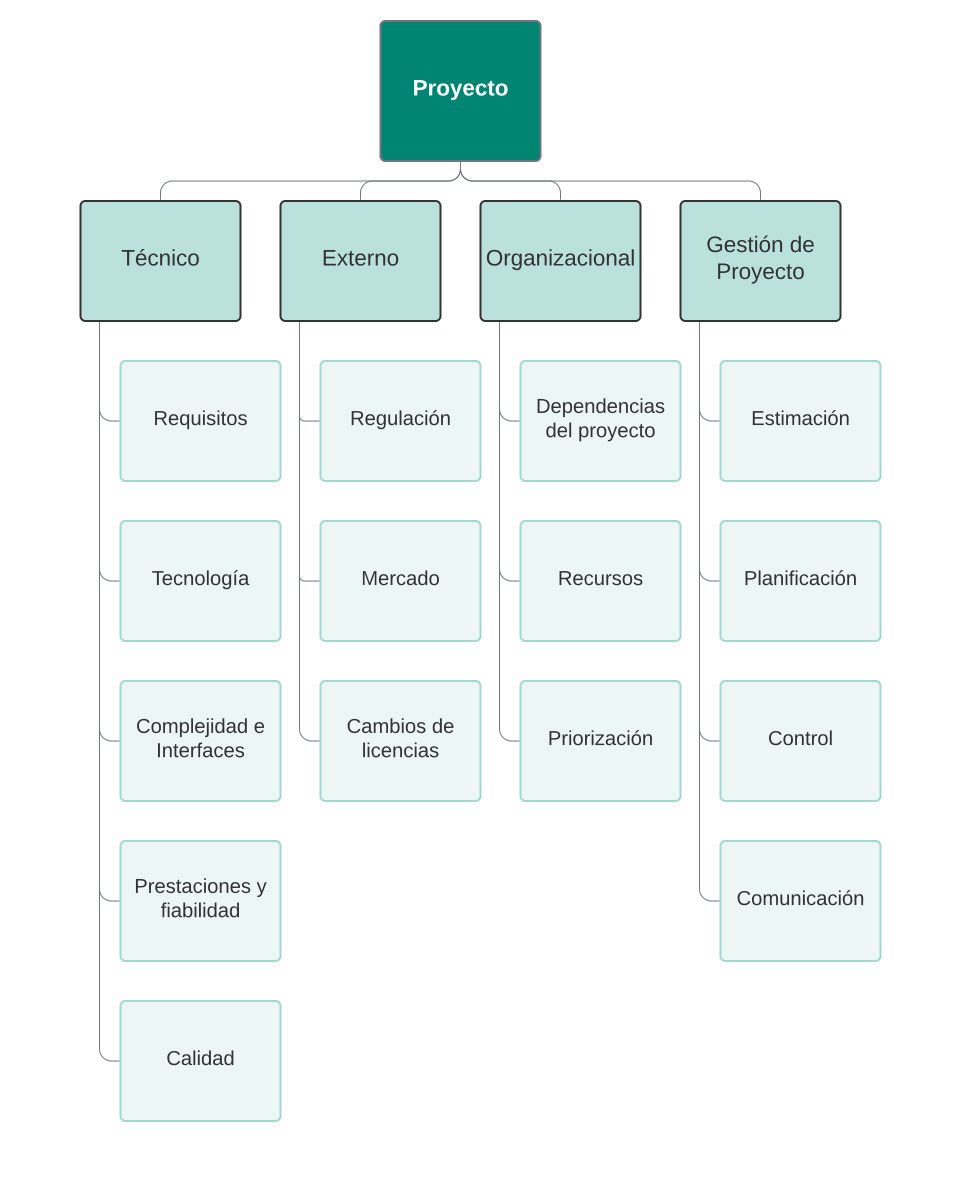
\includegraphics[width=0.65\linewidth]{figures/A1_PGR_RBS.png}
    \caption{RBS, desglose de categorías de riesgos del proyecto}
    \label{fig:A1_PGR_RBS}
\end{figure}

\subsubsection*{Probabilidad e impacto}
Para la valoración de riesgos se ha utilizado una matriz de probabilidad vs impacto, que se muestra en la figura \coloredUnderline{\hyperlink{fig:A1_PGR_matriz_prob_vs_impact}{Matriz de probabilidad vs impacto}}. 
Esta matriz define los valores utilizados en la priorización de riesgos. Cada riesgo tendrá un valor asociado de acuerdo a la probabilidad de que ocurra y el impacto que tendría en el proyecto si ocurriera.

\begin{figure}[H]
    \hypertarget{fig:A1_PGR_matriz_prob_vs_impact}{}
    \centering
    \includegraphics{figures/A1_PGR_matriz_prob_vs_impact.png}
    \caption{Matriz de probabilidad vs impacto}
    \label{fig:A1_PGR_matriz_prob_vs_impact}
\end{figure}

\subsubsection*{Identificación de riesgos}
Para la identificación de riesgos se han utilizado dos técnicas principales: la recopilación de información mediante \textit{brainstorming} y, de forma complementaria, el análisis de listas de control. La combinación de estas técnicas ha permitido una identificación de riesgos realista, abarcando tanto los riesgos inherentes al tipo de proyecto, es decir, desarrollo de software, como los riesgos específicos del proyecto en particular.

\subsubsection*{Análisis de riesgos}
Una vez identificados los riesgos, se ha procedido a analizarlos. Se ha llevado a cabo un análisis cualitativo de los riesgos que consta de los siguientes procesos:
\begin{itemize}
    \item \textbf{Evaluación de la probabilidad e impacto de los riesgos.} Se han asignando valores de probabilidad e impacto a cada uno de ellos, obteniendo así un valor de prioridad en base a la \coloredUnderline{\hyperlink{fig:A1_PGR_matriz_prob_vs_impact}{matriz de probabilidad vs impacto}}.
    \item \textbf{Categorización de riesgos:} Se categorizan los riesgos en función de las \coloredUnderline{\hyperlink{fig:A1_PGR_RBS}{categorías de riesgos}} identificadas.
    \item \textbf{Evaluación de la urgencia de los riesgos:} Se realiza una primera priorización de los riesgos en base a la urgencia con la que deben ser tratados.
\end{itemize}


\subsubsection*{Priorización}
Una vez analizados los riesgos, se ha procedido a priorizarlos. Para ello, se ha utilizado la \coloredUnderline{\hyperlink{fig:A1_PGR_matriz_prob_vs_impact}{matriz de probabilidad vs impacto}}, asignando a cada riesgo un valor de prioridad. 
De esta manera, se obtiene una lista de riesgos ordenada de mayor a menor importancia, lo que permite centrar los esfuerzos en los riesgos más críticos.

\subsubsection*{Planificación de la gestión de cada riesgo}
Se lleva a cabo un análisis más detallado de los riesgos definiendo las estrategias de respuesta a los mismos. 
En el proyecto se ha optado por las siguientes estrategias de respuesta:
\begin{itemize}
    \item \textbf{Evitar el riesgo:} Se trata de eliminar la amenaza o la oportunidad que representa el riesgo.
    \item \textbf{Transferir el riesgo:} Se trata de trasladar la responsabilidad del riesgo a un tercero.
    \item \textbf{Mitigar el riesgo:} Se trata de reducir la probabilidad de ocurrencia o en caso de que ocurra, reducir el impacto.
    \item \textbf{Aceptar el riesgo:} Se trata de asumir las consecuencias del riesgo y convivir con él.
\end{itemize}

\subsubsection*{Resolución de riesgos}
Una vez planificadas las respuestas a los riesgos, se procede a la resolución de los mismos determinando si los riesgos son eliminados o solucionados. 
En este proyecto la técnica que se ha llevado a cabo ha sido el desarrollo incremental con el fin de minimizar los riesgos y permitir una mayor flexibilidad en la gestión de los mismos.

\subsubsection*{Monitorización y control de riesgos}
Por último, se establece un plan de monitorización y control de riesgos. 
La principal técnica utilizada para la monitorización y control de riesgos son las reuniones periódicas de seguimiento del proyecto, en las que se controla el progreso del proyecto, se revisan los riesgos y se actualiza la información de los mismos tomando las medidas correctoras necesarias en cada momento.
